\documentclass[twocolumn]{IEEEtran}
\usepackage{graphicx}
\usepackage[utf8x]{inputenc}
\usepackage{times}
\usepackage{amssymb,amsfonts}
\usepackage[tbtags]{amsmath}
\usepackage{cite}
\usepackage{pict2e}
\usepackage{float}
\usepackage{lscape}
\usepackage[all]{xy}
\usepackage{graphics,graphicx,color,colortbl}
\usepackage{times}
\usepackage{subfigure}
\usepackage{wrapfig}
%\usepackage{multicol}
\usepackage{cite}
\usepackage{url}
\usepackage[tbtags]{amsmath}
\usepackage{amsmath,amssymb,amsfonts,amsbsy}
\usepackage{listings}
\usepackage{bm}
\usepackage{algorithm}
\usepackage{algorithmic}
\usepackage[centerlast, small]{caption}
\usepackage[colorlinks=true, citecolor=blue, linkcolor=blue, urlcolor=blue, breaklinks=true]{hyperref}
\hyphenation{ele-men-tos he-rra-mi-en-ta cons-tru-yen trans-fe-ren-ci-a pro-pu-es-tas si-mu-lar vi-sua-li-za-cion}

\begin{document}
\title{Comportamiento dinámico y estático de algunas configuraciones CMOS}
\author{Nicolás David Arias Sosa \textbf{Código:} $xxxxxx$ \url{ndariass@unal.edu.co}\\
	David Ricardo Martínez Hernández \textbf{Código:} $261931$ \url{drmartinezhe@unal.edu.co}\\
	Oscar Alejandro Rojas Gallego \textbf{Código:} $xxxxxx$ \url{oarojasg@unal.edu.co}\\
	Universidad Nacional de Colombia}
\markboth{Comportamiento dinámico y estático de algunas configuraciones CMOS.}{}
\maketitle
\begin{abstract}
 Se implementaron las compuertas NAND, OR y una compuerta de transmisión por medio del circuito integrado $CD4007$, a dichas eléctricos compuertas se les caracterizaron los parámetros de operación, con $V_{DD}$ diferentes entre los $5\, V$ y $3\, V$, a demás se midieron las potencias consumidas tanto la estática como la dinámica con $V_{DD}$ diferentes, esto se realizó por medio de criterios explicados en clase. Finalmente se simularon dichas compuertas y se compararon con los valores obtenidos en la práctica.
\end{abstract}
\begin{keywords}
 CMOS, Compuerta, Corte, NAND, NOR, Saturación.
\end{keywords}

\section{Introducción}

\subsection{Compuerta NAND de dos entradas}
\noindent
Las entradas en nivel alto, hace que los transistores $Q_{P1}$ y $Q_{P2}$ entren en corte y los transistores $Q_{N1}$ y $Q_{N2}$ en conducción (TABLA \ref{tab1}). La salida pasa a bajo o $0$ a través de $Q_{N1}$ y $Q_{N2}$.\\
Cuando ambas entradas están en bajo, $Q_{P1}$ y $Q_{P2}$ entran a conducción y $Q_{N1}$ y $Q_{N2}$ entran a corte.\\
En las parejas de transistores ya sean de canal n ó de canal p, si cualquier entrada es baja, uno de los transistores entra a corte y otro a conducción.
\begin{figure}[H]
  \centering
    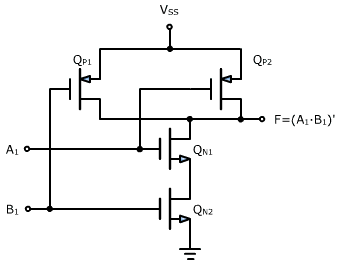
\includegraphics[scale=0.5]{fig1.png}
      \caption{Compuerta NAND. Tomada de \cite{page1}.}
	\label{fig1}
\end{figure}
\begin{table}[H]
  \caption{Tabla de salida y operación}
    \centering
      \begin{tabular}{|c|c|c|c|c|c|c|}\hline
      $A_1$ & $B_1$ & $Q_{P1}$ & $Q_{P2}$ & $Q_{N1}$ & $Q_{N2}$ & $F$ \\ \hline
      $0$ & $0$ & \bf ON & \bf ON & \bf OFF & \bf OFF & 1 \\ \hline
      $0$ & $1$ & \bf ON & \bf OFF & \bf OFF & \bf ON & 1 \\ \hline
      $1$ & $0$ & \bf OFF & \bf ON & \bf ON & \bf OFF & 1 \\ \hline
      $1$ & $1$ & \bf OFF & \bf OFF & \bf ON & \bf ON & 0 \\ \hline
      \end{tabular}
  \label{tab1}
\end{table}

\subsection{Compuerta NOR de dos entradas}
\noindent
Las entradas en nivel alto, hacen que los transistores $Q_{P1}$ y $Q_{P2}$ entren en corte y ambos transistores $Q_{N1}$ y $Q_{N2}$ en conducción (TABLA \ref{tab2}). La salida pasa a bajo o $0$ a través de $Q_{N1}$ y $Q_{N2}$.\\
Cuando ambas entradas están en bajo, $Q_{P1}$ y $Q_{P2}$ entran a conducción y $Q_{N1}$ y $Q_{N2}$ entran a corte.\\
En las parejas de transistores ya sean de canal n ó de canal p, si cualquier entrada es baja, uno de los transistores entra a corte y otro a conducción.
\begin{figure}[H]
  \centering
    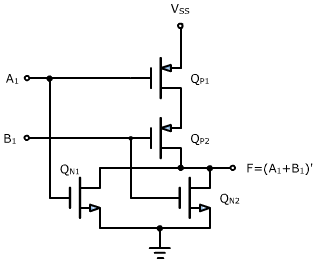
\includegraphics[scale=0.5]{fig2.png}
      \caption{Compuerta NOR. Tomada de \cite{page1}.}
	\label{fig2}
\end{figure}
\begin{table}[H]
  \caption{Tabla de salida y operación}
    \centering
      \begin{tabular}{|c|c|c|c|c|c|c|}\hline
      $A_1$ & $B_1$ & $Q_{P1}$ & $Q_{P2}$ & $Q_{N1}$ & $Q_{N2}$ & $F$ \\ \hline
      $0$ & $0$ & \bf ON & \bf ON & \bf OFF & \bf OFF & 1 \\ \hline
      $0$ & $1$ & \bf ON & \bf OFF & \bf OFF & \bf ON & 0 \\ \hline
      $1$ & $0$ & \bf OFF & \bf ON & \bf ON & \bf OFF & 0 \\ \hline
      $1$ & $1$ & \bf OFF & \bf OFF & \bf ON & \bf ON & 0 \\ \hline
      \end{tabular}
  \label{tab2}
\end{table}

\subsection{Compuerta de transmisión}
\noindent
La compuerta de transmisión es un dispositivo utilizado como interruptor controlado por tensión. Generalmente se emplean transistores para cumplir la función de interrupción y existen compuertas en tecnología NMOS, PMOS y CMOS.

\subsubsection{Compuerta de transmisión NMOS}
\noindent
La compuerta \textbf{NMOS} corresponde a un transistor \textbf{MOS de canal N} Fig. \ref{fig3}. Se observa que la fuente se encuentra conectada a tierra. Este transistor puede conducir corriente en cualquiera de sus dos direcciones cuando la tensión en la compuerta supere la tensión de umbral para encenderlo, aplicando un $1$ lógico.
\begin{figure}[H]
  \centering
    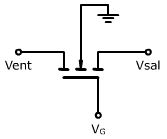
\includegraphics[scale=0.7]{fig3.png}
      \caption{Compuerta de transmisión NMOS. Tomada de \cite{page1}.}
	\label{fig3}
\end{figure}

\subsubsection{Compuerta de transmisión PMOS}
\noindent
El transistor \textbf{MOS de canal P} Fig. \ref{fig4} funciona como compuerta de transmisión. Su funcionamiento es similar a la compuerta de transmisión NMOS, excepto que la lógica que maneja para entrar en conducción es inversa, es decir que la tensión en la compuerta debe ser negativa para encender el transistor, en este caso la señal aplicada corresponde a un $0$ lógico.
\begin{figure}[H]
  \centering
    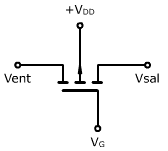
\includegraphics[scale=0.7]{fig4.png}
      \caption{Compuerta de transmisión PMOS. Tomada de \cite{page1}.}
	\label{fig4}
\end{figure}

\subsubsection{Compuerta de transmisión CMOS}
\noindent
Esta compuerta agrupa algunas características de las compuertas de transmisión NMOS y PMOS. En la Fig. \ref{fig5} se ilustra el circuito de esta compuerta, observe que esta compuerta contiene un transistor NMOS, un PMOS y un Inversor.
\begin{figure}[H]
  \centering
    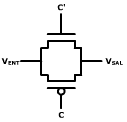
\includegraphics[scale=0.7]{fig5.png}
      \caption{Compuerta de transmisión CMOS. Tomada de \cite{page1}.}
	\label{fig5}
\end{figure}
\noindent
El inversor es empleado para tener una sola señal de control para encender o apagar los transistores. Cuando $V_C$ se encuentra en bajo o $0$ lógico el transistor NMOS se apaga al igual que el transistor PMOS, análogamente, si la tensión $V_C$ cambia a alto o $1$ lógico, los transistores se encienden.

\section{Compuerta NAND de dos entradas}
\noindent
Para la Fig. \ref{fig6} se excito en el PIN $3$ con una onda triangular y en el PIN $6$ con un $1$ lógico.
\begin{figure}[H]
\centering
	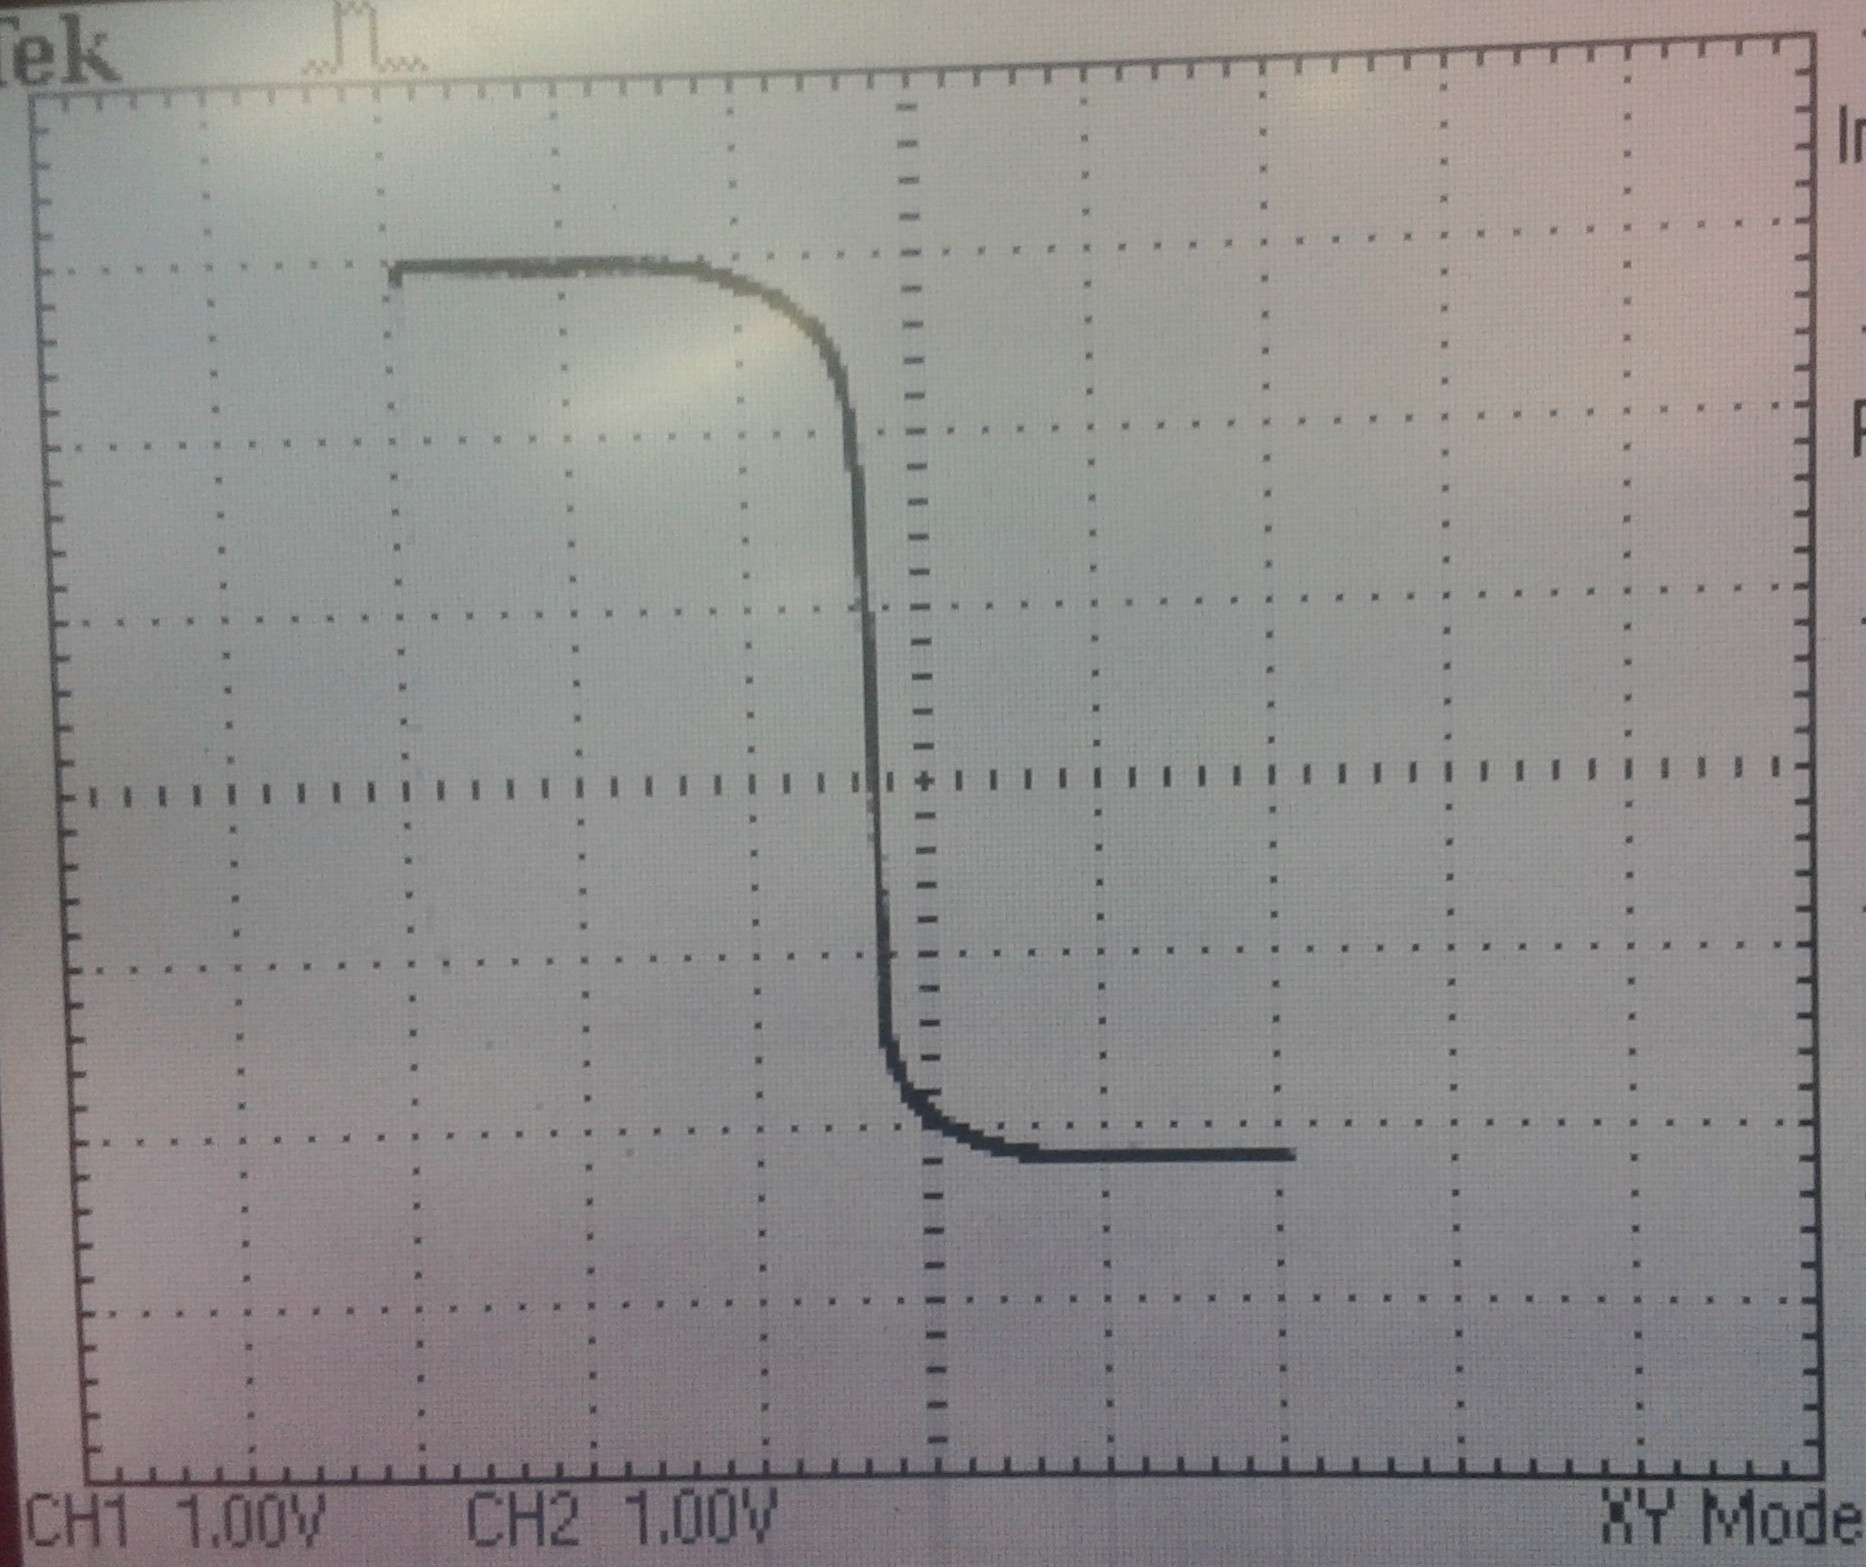
\includegraphics[scale=0.1]{f1.jpg}
	\caption{.}
	\label{fig6}
\end{figure}
\noindent
Los valores de operación de la compuerta NAND se encuentran en la TABLA \ref{tab3}.
\begin{table}[H]
  \centering
    \caption{Tablas de operación compuerta NAND.}
      \begin{tabular}{|c|c|}\hline
      \textbf{Valor} & \textbf{Tiempo ($ns$)} \\ \hline
      $t_r$ & $224$ \\ \hline
      $t_f$ & $308$ \\ \hline
      $t_{plh}$ & $105$ \\ \hline
      $t_{phl}$ & $172$ \\ \hline
      \end{tabular}
  \label{tab3}
\end{table}

\subsection{Potencia estática}
\noindent
La TABLA \ref{tab4} relaciona el consumo de corriente consumido solo por la compuerta polarizada sin carga alguna.
\begin{table}[H]
  \centering
    \caption{Mediciones de voltaje para determinar consumo de potencia estática.}
      \begin{tabular}{|c|c|c|}\hline
      $V_{DD}\, V$ & \multicolumn{2}{c|}{\textbf{5}}\\ \hline
      \textbf{PIN 3} & \textbf{PIN 6} & $I\, \mu A$ \\ \hline
      Open & Open & $215.9$ \\ \hline
      $1$ & Open & $2494$ \\ \hline
      $0$ & Open & $0$ \\ \hline
      Open & $0$ & $0$ \\ \hline
      Open & $1$ & $133$ \\ \hline
      $1$ & $1$ & $0$ \\ \hline
      $0$ & $0$ & $0$ \\ \hline
      $1$ & $0$ & $0$ \\ \hline
      $0$ & $1$ & $0$ \\ \hline
      $V_{DD}\, V$ & \multicolumn{2}{c|}{\textbf{3}} \\ \hline
      \textbf{PIN 3} & \textbf{PIN 6} & $I\, \mu A$ \\ \hline
      Open & Open & $5.8$ \\ \hline
      $1$ & Open & $0$ \\ \hline
      $0$ & Open & $0$ \\ \hline
      Open & $0$ & $0$ \\ \hline
      Open & $1$ & $1.4$ \\ \hline
      $1$ & $1$ & $0$ \\ \hline
      $0$ & $0$ & $0$ \\ \hline
      $1$ & $0$ & $0$ \\ \hline
      $0$ & $1$ & $0$ \\ \hline
      \end{tabular}
   \label{tab4}
\end{table}

\subsection{Potencia dinámica}
\noindent
La TABLA \ref{tab5} relaciona el consumo de voltaje consumido por el condensador $C$ a un voltaje de polarización $V_{DD}$.
\begin{table}[H]
  \caption{Mediciones de voltaje para determinar consumo de potencia dinámica.}
    \begin{tabular}{|l|c|c|c|c|}\hline
      $V_{DD}\, V$ & \multicolumn{2}{c|}{\textbf{5}}  & \multicolumn{2}{c|}{\textbf{3}} \\ \hline
      \textbf{Frecuencia KHz} & 1 & 10 & 1 & 10 \\ \hline
      $V_C\, V$ & $2.783$ & $3.86$ & $2.149$ & $2.64$ \\ \hline
    \end{tabular}
  \label{tab5}
\end{table}

\section{Compuerta NOR de dos entradas}
\noindent
Para la Fig. \ref{fig7} se excito en el PIN $3$ con una onda triangular y en el PIN $6$ con un $1$ lógico.
\begin{figure}[H]
\centering
	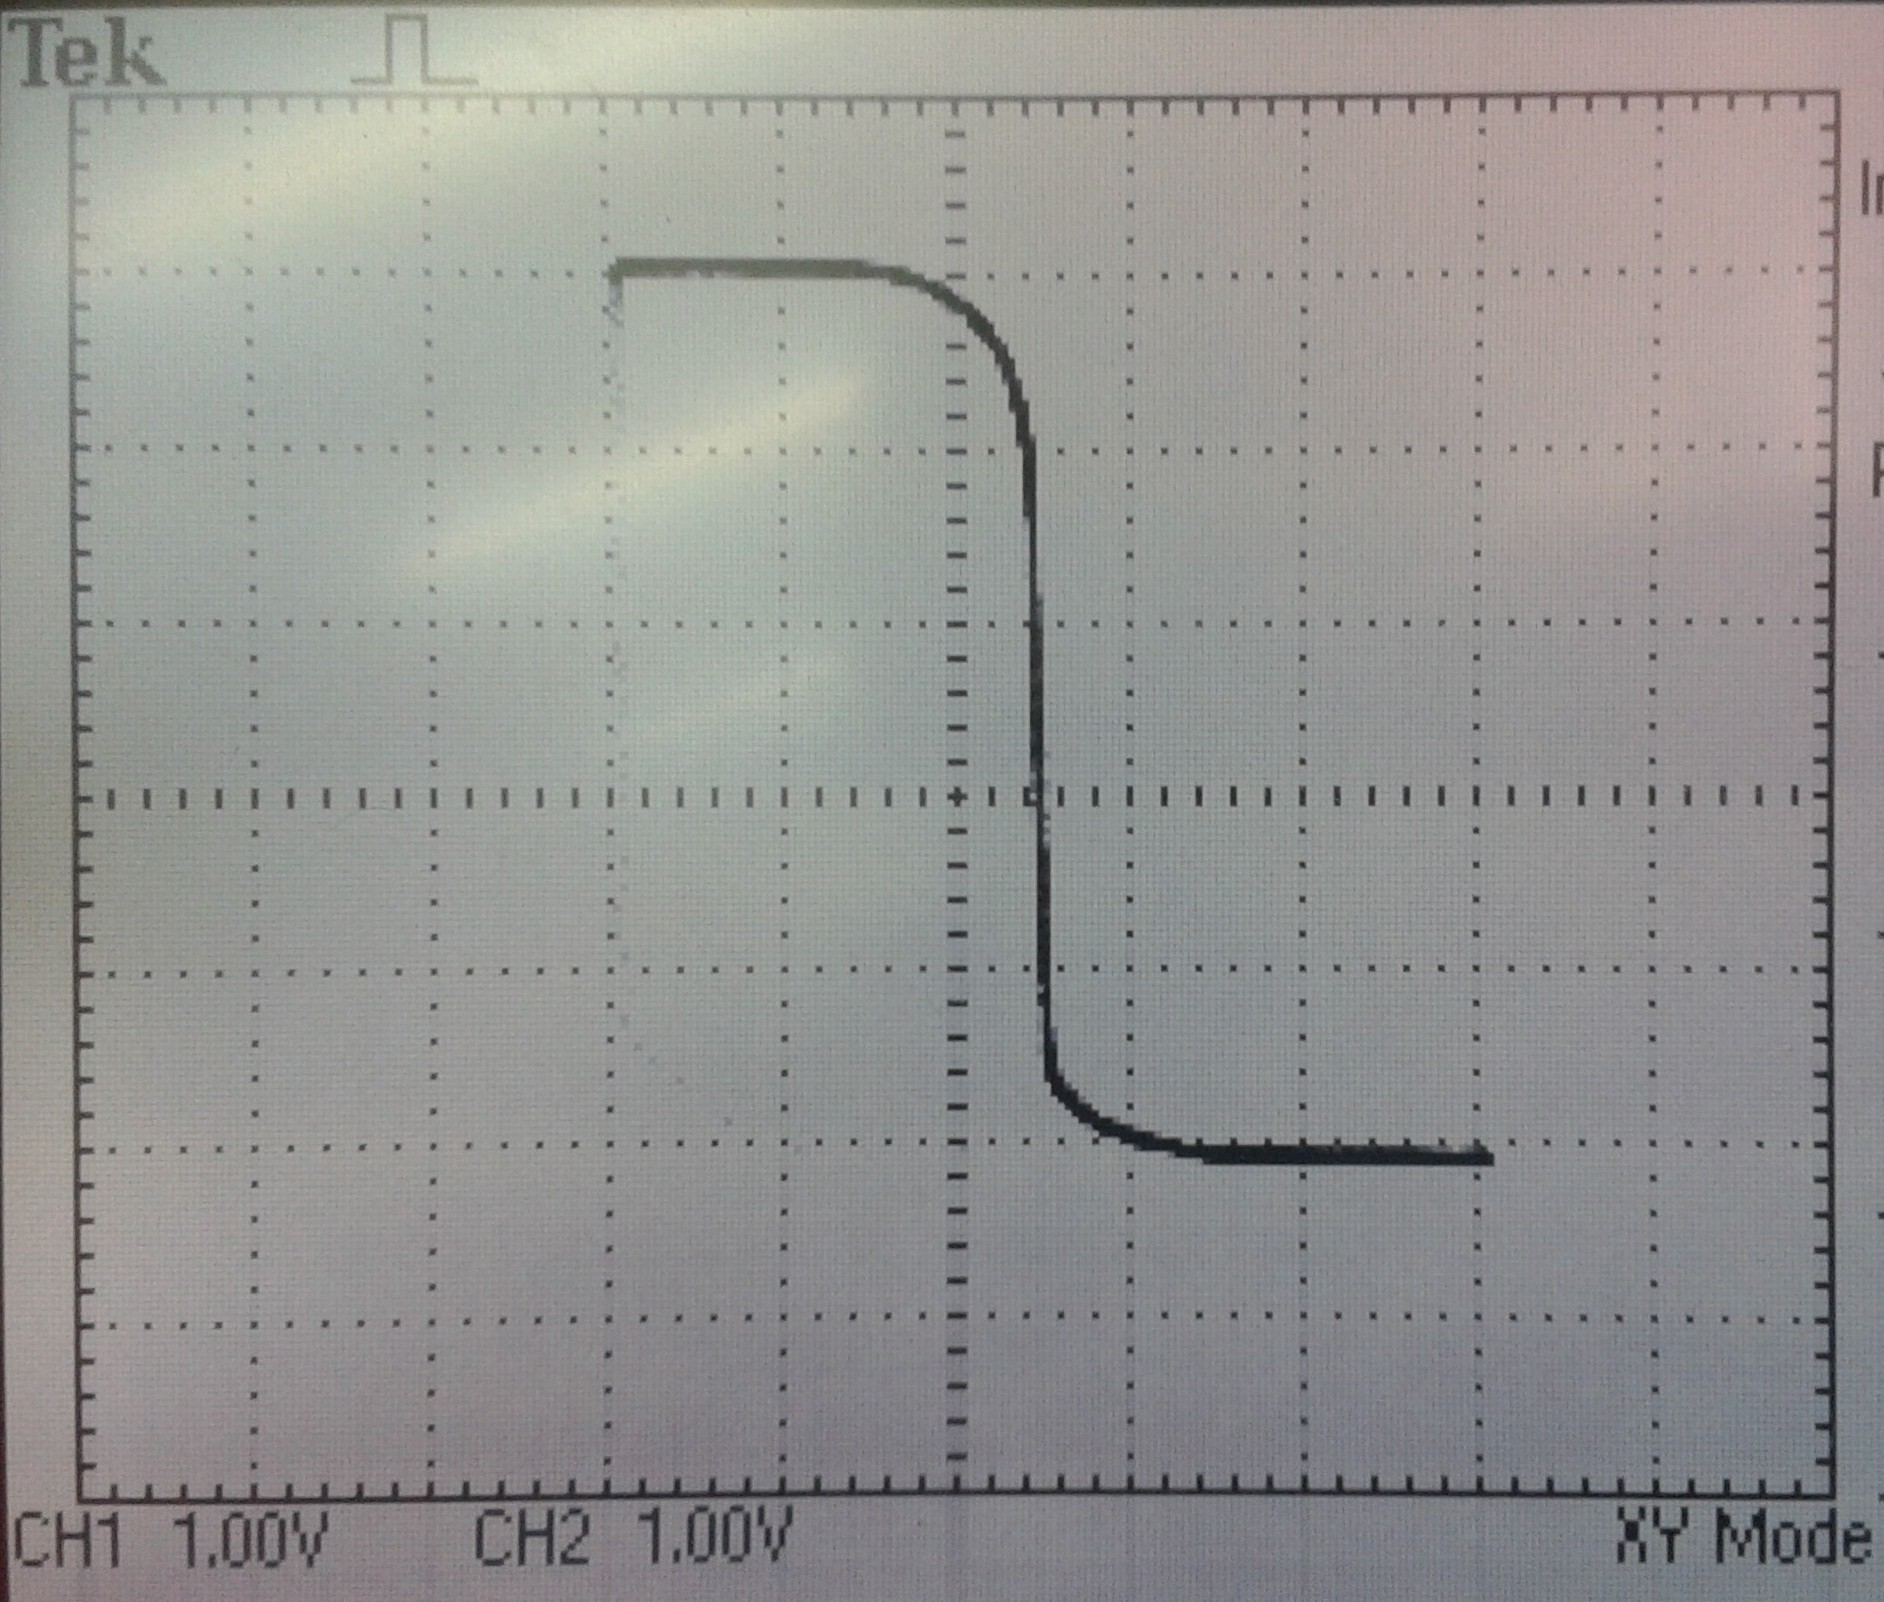
\includegraphics[scale=0.1]{f2.jpg}
	\caption{.}
	\label{fig7}
\end{figure}
\noindent
Los valores de operación de la compuerta NOR se encuentran en la TABLA \ref{tab6}.
\begin{table}[H]
  \centering
    \caption{Tablas de operación compuerta NOR.}
      \begin{tabular}{|c|c|}\hline
      \textbf{Valor} & \multicolumn{1}{l|}{\textbf{Tiempo ($ns$)}} \\ \hline
      $t_r$ & $436$ \\ \hline
      $t_f$ & $168$ \\ \hline
      $t_{plh}$ & $194$ \\ \hline
      $t_{phl}$ & $92$ \\ \hline
      \end{tabular}
  \label{tab6}
\end{table}

\subsection{Potencia estática}
\noindent
La TABLA \ref{tab7} relaciona el consumo de corriente consumido solo por la compuerta polarizada sin carga alguna.
\begin{table}[H]
\centering
  \caption{Mediciones de voltaje para determinar consumo de potencia estática.}
    \begin{tabular}{|c|c|c|}\hline
    $V_{DD}\, V$ & \multicolumn{2}{c|}{\textbf{5}}\\ \hline
    \textbf{PIN 3} & \textbf{PIN 6} & $I\, \mu A$ \\ \hline
    Open & Open & $143$ \\ \hline
    $1$ & Open & $0$ \\ \hline
    $0$ & Open & $213$ \\ \hline
    Open & $0$ & $81$ \\ \hline
    Open & $1$ & $0$ \\ \hline
    $1$ & $1$ & $0$ \\ \hline
    $0$ & $0$ & $0$ \\ \hline
    $1$ & $0$ & $0$ \\ \hline
    $0$ & $1$ & $0$ \\ \hline
    $V_{DD}\, V$ & \multicolumn{2}{c|}{\textbf{3}} \\ \hline
    \textbf{PIN 3} & \textbf{PIN 6} & $I\, \mu A$ \\ \hline
    Open & Open & $2.5$ \\ \hline
    $1$ & Open & $0$ \\ \hline
    $0$ & Open & $3.1$ \\ \hline
    Open & $0$ & $0.7$ \\ \hline
    Open & $1$ & $0$ \\ \hline
    $1$ & $1$ & $0$ \\ \hline
    $0$ & $0$ & $0$ \\ \hline
    $1$ & $0$ & $0$ \\ \hline
    $0$ & $1$ & $0$ \\ \hline
  \end{tabular}
\label{tab7}
\end{table}

\subsection{Potencia dinámica}
\noindent
La TABLA \ref{tab8} relaciona el consumo de voltaje consumido por el condensador $C$ a un voltaje de polarización $V_{DD}$.
\begin{table}[H]
  \caption{Mediciones de voltaje para determinar consumo de potencia dinámica.}
    \begin{tabular}{|l|c|c|c|c|}\hline
      $V_{DD}\, V$ & \multicolumn{2}{c|}{\textbf{5}}  & \multicolumn{2}{c|}{\textbf{3}} \\ \hline
      \textbf{Frecuencia KHz} & $1$ & $10$ & $1$ & $10$ \\ \hline
      $V_C\, V$ & \textbf{Variable} & $0.765$ & $0.332$ & $0.928$ \\ \hline
    \end{tabular}
  \label{tab8}
\end{table}

\section{Análisis de resultados y conclusiones}
\noindent
En la TABLA \ref{tab3} se observan los parámetros físicos o tiempos de respuesta de la compuerta NAND $CD4001$, se encuentran entre los rangos típicos. No hay un retardo considerable dado que las medidas que se tomaron fueron muy imprecisas por los instrumentos de medida que se estaban utilizando, a demás los cursores se ajustaban de acuerdo a como se creía que era el punto de medida adecuado.\\\\
En la TABLA \ref{tab6} se observan los parámetros físicos o tiempos de respuesta de la compuerta NOR $CD4011$, al igual que el análisis anterior las medidas se tomaron de acuerdo a como se creía que era el punto adecuado, aunque no se aleja por mucho de los valores típicos.\\\\
Cuando se estaban tomando las medidas de el consumo de potencia estática se presentaron varios inconvenientes porque no se sabia si debía dejar las terminales de entrada abiertas o se debían llevar a algún estado lógico, aunque se tomaron todas las posibles combinaciones se pudo comprobar que solo había un consumo de corriente considerable en la compuerta NAND cuando se dejaban los pines de entrada como cables al aire con los dos valores de $V_{DD}$. Se determino que la potencia consumida por la compuerta NAND es aproximadamante $1.0795\, mW$ a $V_{DD}=5\, V$ y $17.4\,\mu W$ a $V_{DD}=3\, V$.\\\\
Con la compuerta NOR sucedió algo muy similar pero a diferencia del caso anterior hubo un consumo considerable de corriente cuando se tenían las combinaciones $1$, $3$ o $4$, como en el análisis anterior solo se tomara la potencia cuando las entradas se encuentran abiertas. Se determino que la potencia consumida por la compuerta NOR es aproximadamante $715\,\mu W$ a $V_{DD}=5\, V$ y $7.5\,\mu W$ a $V_{DD}=3\, V$.\\\\
La potencia estática consumida por ambas compuertas se determino por la ecu (\ref{ecu1})
\begin{equation}
 P_{static}=C*f_{conmmutation}*{V_{DD}}^{2}
\label{ecu1}
\end{equation}
\noindent
Dando como resultado para la compuerta NAND se puede observar en la TABLA \ref{tab9}:
\begin{table}[H]
  \caption{Calculo de potencia dinámica.}
    \begin{tabular}{|l|c|c|c|c|}\hline
      $V_{DD}\, V$ & \multicolumn{2}{c|}{\textbf{5}}  & \multicolumn{2}{c|}{\textbf{3}} \\ \hline
      \textbf{Frecuencia KHz} & $1$ & $10$ & $1$ & $10$ \\ \hline
      $P_{static}\,mW$ & $0.25$ & $2.5$ & $0.09$ & $0.9$ \\ \hline
    \end{tabular}
  \label{tab9}
\end{table}
\noindent
Dando como resultado para la compuerta NOR se puede observar en la TABLA \ref{tab10}:
\begin{table}[H]
  \caption{Calculo de potencia dinámica.}
    \begin{tabular}{|l|c|c|c|c|}\hline
      $V_{DD}\, V$ & \multicolumn{2}{c|}{\textbf{5}}  & \multicolumn{2}{c|}{\textbf{3}} \\ \hline
      \textbf{Frecuencia KHz} & $1$ & $10$ & $1$ & $10$ \\ \hline
      $P_{static}\,mW$ & \textbf{Variable} & $2.5$ & $0.09$ & $0.9$ \\ \hline
    \end{tabular}
  \label{tab10}
\end{table}

\bibliographystyle{ieeetran}
\begin{thebibliography}{99}
   
  \bibitem{jeager} Jaeger, Richard C. \& Blalock, Travis N.
  {\em "`Microelectronic Circuit Desing"'}.
  McGraw-Hill, Fourth Edition, 1999.
  
  \bibitem{sedra} Sedra, Adel S. \& Smith, Kenneth C.
  {\em "`Circuitos Microelectrónicos"'}.
  Oxford University Press, Cuarta Edición, 1999.
   
  \bibitem{cd4007} Fairchild Semiconductor. CD4007C -- Dual complementary pair plus inverter. \url{http://cva.stanford.edu/classes/cs99s/datasheets/CD4007C.pdf}
   
  \bibitem{page1} Universidad Nacional de Colombia sede Bogotá, Dirección Nacional de innovación Académica, Electrónica Digital I   \url{http://www.virtual.unal.edu.co/cursos/ingenieria/2000477/lecciones/090501.htm}

  \bibitem{page2} Universidad Nacional de Colombia sede Bogotá, Dirección Nacional de innovación Académica, Electrónica Digital I   \url{http://www.virtual.unal.edu.co/cursos/ingenieria/2000477/lecciones/090301.htm}
  
  \bibitem{page4} Sigma Electrónica LTDA, Manuales de Referencia \url{http://www.sigmaelectronica.net/manuals/CD4001.pdf}
  
\end{thebibliography}
\end{document}